\subsubsection{Extension 3}
\begin{namedframe}{Intersecting}
	\begin{example}
		Show that the Star Trek theorem is still true if the point $C$ is chosen so that $AB$ and $OB$ intersect.

		Prove that $\angle AOC = 2 \angle ACB$.
	\end{example}
	\centering
	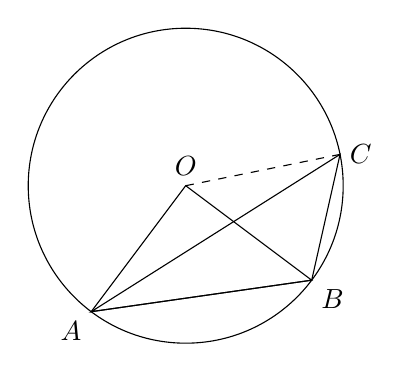
\begin{tikzpicture}[scale=0.4]
		\coordinate [label=above:$O$](O) at (0,0);
		\coordinate [label=below left:$A$](A) at (-3,-4);
		\coordinate [label=below right:$B$](B) at (4,-3);
		\coordinate [label=right:$C$](C) at (4.9,0.994987437107);

		\draw (O) circle (5);
		\draw (A) -- (B) -- (C) -- cycle;
		\draw (A) -- (B) -- (O) -- cycle;
		\draw [dashed] (O) -- (C);
	\end{tikzpicture}
\end{namedframe}
\begin{namedframe}{Extension 3 proof}
	\begin{proof}[Proof that $\angle AOB = 2\angle ACB $.]
		\begin{textblock}{1}(0,0.1)
			\scriptsize
			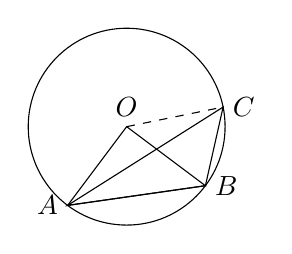
\begin{tikzpicture}[scale=0.25]
				\coordinate [label=above:$O$](O) at (0,0);
				\coordinate [label=left:$A$](A) at (-3,-4);
				\coordinate [label=right:$B$](B) at (4,-3);
				\coordinate [label=right:$C$](C) at (4.9,0.994987437107);

				\draw (O) circle (5);
				\draw (A) -- (B) -- (C) -- cycle;
				\draw (A) -- (B) -- (O) -- cycle;
				\draw [dashed] (O) -- (C);
			\end{tikzpicture}
		\end{textblock}
		\pause
		\begin{equation}\label{eq:ex3:1}
			\angle AOC = \SI{180}{\degree} - 2\angle OCA
		\end{equation}
		\sep[-3ex]
		\begin{equation}\label{eq:ex3:2}
			\angle COB = \SI{180}{\degree} - 2\angle OBC
		\end{equation}
		\sep[-3ex]
		\begin{equation}\label{eq:ex3:3}
			\angle AOB = \angle AOC - \angle COB
		\end{equation}
		\pause
		We can substitute \eqref{eq:ex3:1} and \eqref{eq:ex3:2} into \eqref{eq:ex3:3}:
		\sep[-4ex]
		\begin{align*}
			\angle AOB &= \SI{180}{\degree} - 2\angle OCA - (\SI{180}{\degree} - 2\angle OBC)\\
			\angle AOB &= - 2\angle OCA + 2\angle OBC\\
			\angle AOB &= 2(\angle OBC - \angle OCA)\\
		\end{align*}
		\sep[-4ex]
		We know that know that $\angle ACB = \angle OCB - \angle OCA$.
		\sep[-2ex]
		\[\therefore \angle AOB = 2 \angle ACB \qedhere\]
	\end{proof}
\end{namedframe}
